\documentclass{article}

\usepackage{fancyhdr}
\usepackage{extramarks}
\usepackage{amsmath}
\usepackage{amsthm}
\usepackage{amsfonts}
\usepackage{tikz}
\usepackage[plain]{algorithm}
\usepackage{algpseudocode}
\usepackage[utf8]{inputenc}
\usepackage[T1]{fontenc}
\usepackage{natbib}

\usetikzlibrary{automata,positioning}

%
% Basic Document Settings
%

\topmargin=-0.45in
\evensidemargin=0in
\oddsidemargin=0in
\textwidth=6.5in
\textheight=9.0in
\headsep=0.25in

\linespread{1.1}

\pagestyle{fancy}
%\lhead{\hmwkAuthorName}
%\chead{\hmwkClass\ (\hmwkClassInstructor\ \hmwkClassTime): \hmwkTitle}
\lhead{\hmwkClass: \hmwkTitle}
\rhead{\hmwkAuthorName}
\lfoot{\lastxmark}
\cfoot{\thepage}

\renewcommand\headrulewidth{0.4pt}
\renewcommand\footrulewidth{0.4pt}

\setlength\parindent{0pt}
\setlength{\parskip}{1em}

%
% Create Problem Sections
%

\newcommand{\enterProblemHeader}[1]{
    \nobreak\extramarks{}{Problem \arabic{#1} continued on next page\ldots}\nobreak{}
    \nobreak\extramarks{Problem \arabic{#1} (continued)}{Problem \arabic{#1} continued on next page\ldots}\nobreak{}
}

\newcommand{\exitProblemHeader}[1]{
    \nobreak\extramarks{Problem \arabic{#1} (continued)}{Problem \arabic{#1} continued on next page\ldots}\nobreak{}
    \stepcounter{#1}
    \nobreak\extramarks{Problem \arabic{#1}}{}\nobreak{}
}

\setcounter{secnumdepth}{0}
\newcounter{partCounter}
\newcounter{homeworkProblemCounter}
\setcounter{homeworkProblemCounter}{1}
%\nobreak\extramarks{Problem \arabic{homeworkProblemCounter}}{}\nobreak{}

%
% Homework Problem Environment
%
% This environment takes an optional argument. When given, it will adjust the
% problem counter. This is useful for when the problems given for your
% assignment aren't sequential. See the last 3 problems of this template for an
% example.
%
\newenvironment{homeworkProblem}[1][-1]{
    \ifnum#1>0
        \setcounter{homeworkProblemCounter}{#1}
    \fi
    \section{Problem \arabic{homeworkProblemCounter}}
    \setcounter{partCounter}{1}
    \enterProblemHeader{homeworkProblemCounter}
}{
    \exitProblemHeader{homeworkProblemCounter}
}

%
% Homework Details
%   - Title
%   - Due date
%   - Class
%   - Section/Time
%   - Instructor
%   - Author
%

\newcommand{\hmwkTitle}{Exercices}
\newcommand{\hmwkDueDate}{5 février, 2017}
\newcommand{\hmwkClass}{MTH8408}
\newcommand{\hmwkClassTime}{}
\newcommand{\hmwkClassInstructor}{Professeur Dominique Orban}
\newcommand{\hmwkAuthorName}{André Phu-Van Nguyen}
\renewcommand{\refname}{Références}

%
% Title Page
%

\title{
    \vspace{2in}
    \textmd{\textbf{\hmwkClass:\ \hmwkTitle}}\\
%    \normalsize\vspace{0.1in}\small{Remis\ pour\ le\ \hmwkDueDate\ }\\
%    \vspace{0.1in}\large{\textit{\hmwkClassInstructor\ \hmwkClassTime}}
    \vspace{4in}
}

\author{\textbf{\hmwkAuthorName}}
\date{}

\renewcommand{\part}[1]{\textbf{\large Part \Alph{partCounter}}\stepcounter{partCounter}\\}

%
% Various Helper Commands
%

% Useful for algorithms
\newcommand{\alg}[1]{\textsc{\bfseries \footnotesize #1}}

% For derivatives
\newcommand{\deriv}[1]{\frac{\mathrm{d}}{\mathrm{d}x} (#1)}

% For partial derivatives
\newcommand{\pderiv}[2]{\frac{\partial}{\partial #1} (#2)}

% Integral dx
\newcommand{\dx}{\mathrm{d}x}

% Alias for the Solution section header
\newcommand{\solution}{\textbf{\large Solution}}
\newcommand{\norm}[1]{\left\lVert#1\right\rVert}

% Probability commands: Expectation, Variance, Covariance, Bias
\newcommand{\E}{\mathrm{E}}
\newcommand{\Var}{\mathrm{Var}}
\newcommand{\Cov}{\mathrm{Cov}}
\newcommand{\Bias}{\mathrm{Bias}}
\newcommand{\incomplete}{\textcolor{red}{Incomplete}}

\begin{document}

\maketitle

\pagebreak

\section{Unconstrained Programming Exercices}

\subsection{Problem 1}

Discutez, suivant les valeurs du paramètre $\beta \in \mathrm{R}$, la nature des points stationnaires de la fonction de deux variables
\[
f(x,y) = x^2 + y^2 + \beta xy + x + 2y
\]

\textbf{Answer}
\begin{align*}
\nabla f(x,y) &= 
	\begin{bmatrix}
		2x + \beta y + 1 \\
		2y + \beta x + 2
	\end{bmatrix} \\
\textbf{H}(f(x,y)) &=
	\begin{bmatrix}
		2 & \beta \\
		\beta & 2
	\end{bmatrix}
\end{align*}
Find the eigen values
\begin{align*}
\text{det}(\lambda I - \textbf{H}) &= 0 \\
\text{det}\Bigg( 
	\begin{bmatrix}
		\lambda -2 & -\beta \\
		-\beta & \lambda - 2
	\end{bmatrix}
\Bigg) &= 0 \\
(\lambda -2)^2 - \beta^2 &= 0 \\
\lambda^2 -4\lambda + y - \beta^2 &= 0
\end{align*}
Using the quadratic formula
\begin{align*}
\lambda &= \frac{4 \pm \sqrt{16 - 4 \cdot 1 \cdot (4-\beta^2)}}{2} \\
&= \frac{4 \pm \sqrt{4 \beta^2}}{2} \\
&= \frac{4 \pm 2\beta}{2} \\
&= 2 \pm \beta
\end{align*}

\begin{center}
\begin{tabular}{|c|c|c|}
	\hline
	$\beta < -2$ & $\beta \in [-2, 2]$ & $\beta > 2$ \\
	\hline
	$\lambda_1 < 0$, $\lambda_2 > 0$ & $\lambda_1 = [0, 4]$, $\lambda_2 = [4, 0]$& $\lambda_1 > 0$, $\lambda_2 < 0$\\
	Indefinite matrix & Semi-definite positive matrix & Indefinite matrix\\
	\hline
	Saddle point & local minimum & saddle point \\
	\hline
\end{tabular}
\end{center}

\pagebreak
\subsection{Problem 2}

Soit la minimisation sans contraintes de la fonction
\[
f(x_1,x_2) = 2x_1^2 + x_2^2 -2x_1x_2 + 2x_1^3 + x_1^4
\]
\begin{enumerate}[(a)]
\item Trouvez les candidats solution du problème et pour chacun d’entre eux, précisez s’il s’agit d’un minimum local, d’un maximum local ou d’un point selle. Justifiez vos réponses.
\item Y a-t-il un minimum global dans ce cas? Si oui, lequel?
\end{enumerate}

\textbf{Answer}

\textbf{a)}
\begin{align*}
\nabla f(x_1, x_2) =
\begin{bmatrix}
4x_1 - 2x_2 + 6x_1^2 + 4x_1^3 \\
2x_2 - 2x_1
\end{bmatrix} &= 0\\
2x_2 - 2x_1 &\Rightarrow x_2 = x_1
\end{align*}
Substituting into the first line we get
\begin{align*}
	4x_1^3 + 6x_1^2 + 2x_1 &= 0 \\
	2x_1^3 + 3x_1^2 + x_1 &= 0 \\
	x_1(2x_1+1)(x_1+1) &=0 \\
	x_1 = 0, -1 \text{ or } -\frac{1}{2}
\end{align*}
Our 3 stationary points are $(0,0)$, $(-1,-1)$ and $(-\frac{1}{2}, -\frac{1}{2})$
\begin{align*}
\textbf{H} = 
\begin{bmatrix}
	12x_1^2 + 12x_1 + 4 & -2 \\
	-2 & 2
\end{bmatrix}
\end{align*}
Find the eigen values of the hessian
\begin{align*}
\text{det}(\lambda I - \textbf{H}) &= 0 \\
\text{det}\Bigg( 
\begin{bmatrix}
	\lambda -4(3x_1^2 + 3 x_1 + 1) & -2 \\
	-2 & \lambda -2
\end{bmatrix}
\Bigg) &= 0 \\
\Big(\lambda -4(3x_1^2 + 3 x_1 + 1)\Big)(\lambda -2) -4 &= 0
\end{align*}
For $(x_1, x_2) = (0,0)$ we have
\begin{align*}
	(\lambda-4(0-0+1))(\lambda -2 ) -4 &= 0 \\
	(\lambda -4)(\lambda -2) -4 &= 0 \\
	\lambda^2 - 6\lambda + 4 &= 0 \\
	\lambda &= \frac{6 \pm \sqrt{36 - 4 \cdot 4}}{2} \\
	\lambda &= 3 \pm \sqrt{5} \\
	\lambda_1 > 0, \lambda_2 >0
\end{align*}
Both values of $\lambda$ are positive making the Hessian definite positive at $(0,0)$ making the point a local minimum.

For $(x_1, x_2) = (1,1)$ we have
\begin{align*}
(\lambda-4(3-3+1))(\lambda -2 ) -4 &= 0 \\
(\lambda -4)(\lambda -2) -4 &= 0
\end{align*}
Which goes back to the same answer as above, thus $(1,1)$ is also a local minimum.

For $(x_1, x_2) = (-\frac{1}{2},-\frac{1}{2})$ we have
\begin{align*}
(\lambda-4(-\frac{3}{4} - \frac{6}{4} + \frac{4}{4}))(\lambda -2 ) -4 &= 0 \\
(\lambda +5)(\lambda -2) -4 &= 0 \\
\lambda^2 + 3 \lambda -14 &= 0 \\
\lambda &= \frac{-3 \pm \sqrt{9-4 \cdot 1 \cdot -14}}{2} \\
\lambda &= \frac{-3 \pm \sqrt{65}}{2}
\lambda &= 2.5311, -5.5311
\end{align*}
Meaning the Hessian is indefinite at $(-\frac{1}{2},-\frac{1}{2})$ making it a saddle point.

\subsection{Problem 3}

On dit qu’un ensemble $C \subseteq \mathrm{R}^n$ est convexe si
\[
	\lambda x+(1-\lambda )y \in C\ \ \ \forall \lambda \in [0,1],\ x, y \in C
\]

\textbf{a)} Donnez une interprétation géométrique de cette propriété et tracez un sous-ensemble de $\mathrm{R}^2$ qui n’est pas convexe.

\answer

We have two points $x$ and $y$ in $C$. If we draw a line from $x$ to $y$, the entire line has to always stay in $C$.
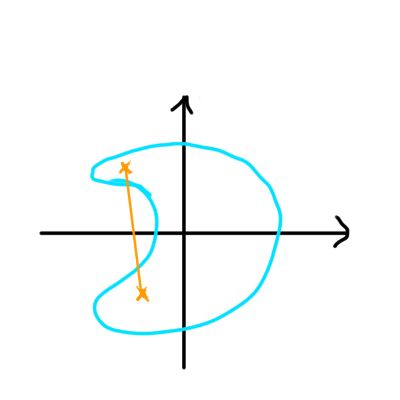
\includegraphics[scale=0.5]{fig/unconstrained_exercices/pb3a.jpg}

\pagebreak
\textbf{b)} 

\answer\footnote{\url{http://ljk.imag.fr/membres/Anatoli.Iouditski/cours/convex/chapitre_3.pdf} page 57}

Let $x,\ y\ \in C_\alpha$, take $f$ of the convex equation
\begin{align*}
f\Big(\lambda x + (1-\lambda)y \Big) &\geq f(\lambda x) + f\Big((1-\lambda)y\Big)
\intertext{Since $f$ is convex we can write by definition that}
f(\lambda x + (1-\lambda)y) &\geq f(\lambda x) + f((1-\lambda)y) \geq \lambda f(x) + (1-\lambda)f(y)
\end{align*}
Since  $x,\ y\ \in C_\alpha$ we can write
\[
f(\lambda x + (1-\lambda)y) \geq \lambda \alpha + (1-\lambda) \alpha
\]
Which is the same as
\[
f(\lambda x + (1-\lambda)y) \geq \alpha
\]
Thus $C_\alpha$ is convex
\textbf{c)}

\answer

The epigraph is the volume on top of a curve, including the curve itself. So we choose two points $(x_1, t_1)$ and $(x_2, t_2)$ both $\in \text{epi}(f)$ meaning that
\begin{align*}
	f(x_1) &\leq t_1 \\
	f(x_2) &\leq t_2
\end{align*}
To show that epi$(f)$ is convex we need to show that
\[
\lambda(x_1, t_1) + (1-\lambda)(x_2,t_2) \in \text{epi}(f)
\]
We can rewrite the lhs as the point
\[
\Big(\lambda x_1 + (1-\lambda) x_2,\ \lambda t_1 + (1-\lambda) t_2\Big) \in \text{epi}(f)
\]
which would mean that the value of $f$ from $x_1$ to $x_2$ should be less than the line $t_1$ to $t_2$ for any $\lambda \in [0, 1]$ i.e.
\[
f(\lambda x_1 + (1-\lambda) x_2) \overset{?}{\leq} \lambda t_1 + (1-\lambda) t_2
\]
Since $f$ is convex we can write
\[
f(\lambda x_1 + (1-\lambda) x_2) \leq\ \lambda f(x_1) + (1-\lambda)f(x_2) \ \leq \lambda t_1 + (1-\lambda) t_2
\]
which means the previous equation is true, thus epi$(f)$ is convex.

\textbf{d)}

\answer

We want to show that for two points $x_1,\ x_2 \in M$ we have
\[
\lambda x_1 + (1-\lambda)x_2 \in M
\]
We can do this by showing that the linear combination of $x_1$ and $x_2$ is still a minimum of $f$.
\[
f(\lambda x_1 + (1-\lambda)x_2) \overset{?}{\leq} f(x)\ \ \ \ \forall x
\]
Since $f$ is convex we can write
\[
\lambda f(x_1) + (1-\lambda)f(x_2) \overset{?}{\leq} f(x)
\]
But since $x_1$ and $x_2$ are both global minima of $f$ then $f(x_1) = f(x_2)$ and we can write
\begin{align*}
\big(\lambda + (1-\lambda)\big)f(x_1) &\overset{?}{\leq} f(x) \\
f(x_1) &\overset{?}{\leq} f(x)
\end{align*}
Which is true since we know $x_1$ is a global minimum. Thus the set $M$ is convex.

\textbf{e)}

\answer

Use the second order convex definition:

If $f \in \mathcal{C}^2$, $f$ is convex if $\nabla^2 f(x) \succeq 0$

\begin{align*}
	f(x) &= \frac{1}{2} \| Ax-b\|^2 \\
	&= \frac{1}{2} (Ax-b)^T(Ax-b) \\
	&= \frac{1}{2} (x^TA^TAx - 2b^TAx + b^Tb) \\
\end{align*}
Using the identity $\frac{\partial x^T A x}{\partial x} = 2Ax$ we get
\begin{align*}
	\nabla f(x) &= \frac{1}{2} (2A^TAx - 2(b^TA)^T) \\
	&= A^TAx - A^Tb
\end{align*}
Differentiating again we get
\[
	\nabla^2 f(x) = A^TA
\]
Multiplying a matrix by its transpose would make all of it's eigen values squared (and positive). So we know $\nabla^2 \succ 0$, meaning it's convex.


\color{red}
Alternate solution

We know that $f(x) = x^2$, $g(x) = \|x\|$ and $h(x) = Ax-b$ are all convex functions and we know that compositions of convex functions are also convex. Therefore $\frac{1}{2} \| Ax-b\|^2$ is convex.

\color{black}

\subsection{Problem 4}

\textbf{a)}

\answer

Go back to the taylor expansion where
\[
	f(x+h) = f(x) + \nabla f(x)^Th + \text{o}(\| h\|)
\]

So we apply this to $f(x)$ which gives

\begin{align*}
	\frac{1}{2} \| F(x+h) \|^2 &= \frac{1}{2} \| F(x) + \nabla F(x)^Th + \text{o}(\| h\|) \|^2 \\
\intertext{Recall the identity $\| a + b + c\|^2 = \|a\|^2 + \|b\|^2 + \|c\|^2 + 2<a,b> + 2<a,c> + 2<b,c>$}
	&= \frac{1}{2} \|  F(x)\|^2 \textcolor{red}{+ \frac{1}{2} \|  \nabla F(x)^Th\|^2 + \text{o}(\| h\|)^2}
		+ F(x)^T \nabla F(x)^Th \textcolor{red}{+ F(x)o(\|h\|) + \nabla F(x)^ThF(x)o(\|h\|)}
\end{align*}

All the red terms above are basically the error term of the Taylor expansion. By inspection we can then see that 
\begin{align*}
	\nabla f(x)^T &= F(x)^T\nabla F(x)^T \\
	\nabla f(x) &= \nabla F(x)F(x)
\end{align*}


Where if we suppose $F: \mathbb{R}^n \rightarrow \mathbb{R}^n$ then

\[
F(x_1, \ldots, x_n) =
\begin{bmatrix}
	F_1(x_1, \ldots, x_n) \\
	\vdots \\
	F_n(x_1, \ldots, x_n)
\end{bmatrix}
\]

and

\[
\nabla F(x) =
\begin{bmatrix}
	\frac{\partial F_1}{\partial x_1} & \frac{\partial F_2}{\partial x_1} & \ldots & \frac{\partial F_n}{\partial x_1} \\
	\frac{\partial F_1}{\partial x_2} & \\
	\vdots \\
	\frac{\partial F_1}{\partial x_n} & \ldots & & \frac{\partial F_n}{\partial x_n}
\end{bmatrix}
\]


\textbf{b)}

We then have a set of matrices where $i = 1, \ldots , n$

\[
\nabla^2 F_i(x) =
\begin{bmatrix}
\frac{\partial F_1}{\partial x_1 x_1} & \frac{\partial F_1}{\partial x_1 x_2} & \ldots & \frac{\partial F_1}{\partial x_1 x_n} \\
\frac{\partial F_1}{\partial x_2 x_1} & \\
\vdots \\
\frac{\partial F_1}{\partial x_n x_1} & \ldots & & \frac{\partial F_1}{\partial x_n x_n}
\end{bmatrix},
\begin{bmatrix}
\frac{\partial F_i}{\partial x_1 x_1} & \frac{\partial F_i}{\partial x_1 x_2} & \ldots & \frac{\partial F_i}{\partial x_1 x_n} \\
\frac{\partial F_i}{\partial x_2 x_1} & \\
\vdots \\
\frac{\partial F_2}{\partial x_n x_1} & \ldots & & \frac{\partial F_2}{\partial x_n x_n}
\end{bmatrix},\ \ldots,\
\begin{bmatrix}
\frac{\partial F_n}{\partial x_1 x_1} & \frac{\partial F_n}{\partial x_1 x_2} & \ldots & \frac{\partial F_n}{\partial x_1 x_n} \\
\frac{\partial F_n}{\partial x_2 x_1} & \\
\vdots \\
\frac{\partial F_n}{\partial x_n x_1} & \ldots & & \frac{\partial F_n}{\partial x_n x_n}
\end{bmatrix}
\]

Which allows us to describe the Hessian of $f(x)$  as
\begin{align*}
\nabla^2 f(x) &= (F(x) \nabla F(x))' \\
&= \nabla F(x) \nabla F(x)^T + F(x) \nabla^2 F(x) \\
&= \nabla F(x) \nabla F(x)^T + \sum_{i=0}^n F_i(x) \nabla^2F_i(x)
\end{align*}

Which then allows us to say that the descent direction $d$ is
\begin{align*}
	d &= - (\nabla^2 f(x))^{-1} \nabla f(x) \\
	  &= - \Bigg(\nabla F(x) \nabla F(x)^T + \sum_{i=0}^n F_i(x) \nabla^2F_i(x) \Bigg)^{-1} F(x) \nabla F(x)
\end{align*}


\textbf{c)}

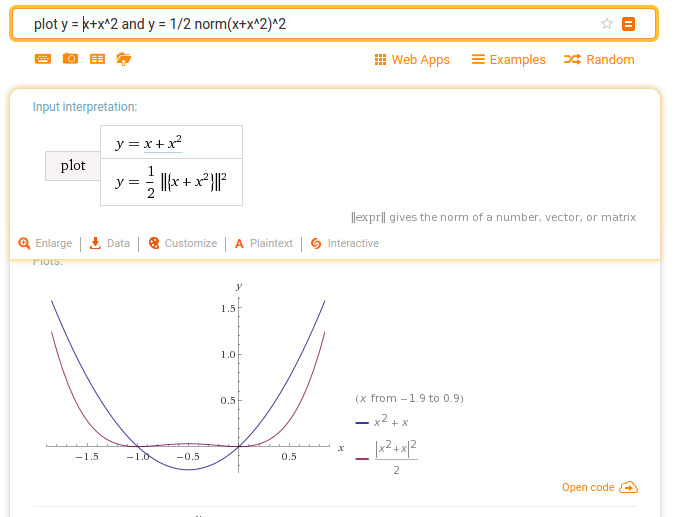
\includegraphics[width=0.6\linewidth]{fig/unconstrained_exercices/pb4_c.png}

We can see there will be 3 critical points including one that doesn't give the right solution to $x+x^2 = 0$.

\subsection{Problem 5}

\[
f(x_1, x_2) = 2x_1^2 -2x_1x_2 + x_2^2 + 2x_1 -2x_2
\]

Apply the steepest descent method with no linesearch starting at $(x_1, x_2) = (0,0)$

\answer

Find the gradient

\[
	\nabla f(x_1, x_2) = 
	\begin{bmatrix}
		4x_1 - 2x_2 + 2 \\
		-2x_1 + 2x_2 - 1	
	\end{bmatrix}
\]

\begin{enumerate}
\item $x_0 = (0,0)$, $k = 0$
\item $d_0 = - \nabla f((0,0)) = - \begin{bmatrix}
2 \\
1
\end{bmatrix}$
\item $x_1 = x_0 + d_k$ \\
$x_1 = \begin{bmatrix}
0 \\ 0
\end{bmatrix} - \begin{bmatrix}
2 \\ 1
\end{bmatrix} = (-2,\ -1)$
\end{enumerate}

Since there is a minimum at $(0,\ 1)$ it is clear that we went in the wrong direction. It is also clear that we went that way by a lot, so this method might never converge.

\subsection{Problem 6}

\incomplete

\subsection{Problem 7}

\textbf{a)}

\begin{lstlisting}[style=Matlab-editor]
function [f, g, H] = obj1(point)
% obj1 First objective function
% f_1(x,y_ = 2x^3 - 3x^2 -6xy(x-y-1)
% Inputs
%   x   Point at which to evaluate the function
% Output
%   f   Result of the function evaluated at x
%   g   Result of the gradient evaluated at x
%   H   Result of the Hessian evaluated at x

x = point(1);
y = point(2);

% function
f = 2*x^3 - 3*x^2 - 6*x*y*(x-y-1);

% gradient
g = [   6 * (x^2 -x -2*x*y +y^2 +y);
        6*x*(2*y - x + 1)];

% hessian
H = [   12*x-12*y-6,        12*y - 12*x + 6; ...
        12*y - 12*x + 6,    12*x];

\end{lstlisting}


\begin{lstlisting}[style=Matlab-editor]
function [f, g, H] = obj2(x)
% obj2 Second objective function if problem 7
%   
% Inputs
%   x   Point at which to evaluate the function
% Output 
%   f   Result of the function evaluated at x
%   g   Result of the gradient evaluated at x
%   H   Result of the Hessian evaluated at x
% Author: Andre Phu-Van Nguyen <andre-phu-van.nguyen@polymtl.ca>

f = 0;
n = length(x) - 1;
for i = 1:n
    tmp = 100 * (x(i+1) - x(i)^2)^2 + (1-x(i))^2;
    f = f + tmp;
end

g = zeros(n, 1);
for i = 1:n
    g(i) = -400 * x(i) * (x(i+1)-x(i)^2) + 2 * (1-x(i));
end


H = zeros(n, n);
for i = 1:n
    % iterate only on the diagonal
    H(i,i) = -400 * x(i+1) + 1200 * x(i)^2 -2;
    if i ~= n
        % Last row doesn't have this term
        H(i,i+1) = -400 * x(i);
    end        
end
\end{lstlisting}

\textbf{b)}

\begin{lstlisting}[style=Matlab-editor]
function [t] = armijo(x, d, obj)
% armijo Armijo line search for problem 7
%   
% Inputs
%   x   Point at which to do the line search
%   d   Direction in which to do the line search
%   obj Objective function we want to optimize
% Output 
%   t   Step length from 0 to 1
% Author: Andre Phu-Van Nguyen <andre-phu-van.nguyen@polymtl.ca>
%
% Theory
% See slides 19/71 take a big step length and shorten it until the armijo 
% condition is satisfied. The Armijo condition is basically that the new 
% step length should make us go somewhere where the function value is 
% smaller than if we had taken a full step.

% full step value
t = 1;
alpha = 0.5;
[armijo, ~] = obj(x + t*d);

% right hand side
[fx, gradx, ~] = obj(x);
rhs = fx + alpha * t * gradx' * d;

while (armijo > rhs) && (t > 10*eps) 
    t = t/2;
    rhs = fx + alpha * t * gradx' * d;
    [armijo, ~] = obj(x + t*d);
end

end
\end{lstlisting}

\textbf{c)}
\begin{lstlisting}[style=Matlab-editor]
function [x_all, convergence] = steepest(x0, obj, verbose)
% steepest Steepest descrnt method with armijo linesearch for problem 7
%   
% Inputs
%   x0  Point at which to start
%   obj Objective function we want to optimize
%   verbose Print out the iterations
% Output 
%   x   End point
% Author: Andre Phu-Van Nguyen <andre-phu-van.nguyen@polymtl.ca>

if nargin > 3
    error('steepest too many inputs')
end

switch nargin
    case 2
        verbose = false;
end

epsilon_a = 0.001;
epsilon_r = 0.001;
max_iter  = 20;
x = x0;
[~, gxk, ~] = obj(x);   % gxk gradient at x_k
[~, gx0, ~] = obj(x0);  % gx0 gradient at x_0

if verbose
    fprintf('k\tf(x)\t\tt_k\tx1\tx2\n');
end

i = 0;
convergence = [];
x_all = [];
while   (norm(gxk) > epsilon_a + epsilon_r*norm(gx0)) && (i < max_iter)
    [f, gxk, ~] = obj(x);
    d_k = -gxk;
    tk = armijo(x, d_k, obj);
    
    if verbose
        g=sprintf('%2.2f ', x);
        fprintf('%d\t %4.4f\t %1.4f\t %s\n', i, f, tk, g);
    end
    
    convergence = [convergence f];
    x_all = [x_all x];
    x = x + tk * d_k;
    i = i + 1;
    
end
\end{lstlisting}

\textbf{d)}
\begin{lstlisting}[style=Matlab-editor]
function [x_all, convergence] = newton(x0, obj, verbose)
% newton Newton descent method with armijo linesearch for problem 7
%   
% Inputs
%   x0  Point at which to start
%   obj Objective function we want to optimize
%   verbose Print out the iterations
% Output 
%   x   End point
% Author: Andre Phu-Van Nguyen <andre-phu-van.nguyen@polymtl.ca>

if nargin > 3
    error('steepest too many inputs')
end

switch nargin
    case 2
        verbose = false;
end

epsilon_a = 0.001;
epsilon_r = 0.001;
max_iter  = 20;
x = x0;
[~, gxk, ~] = obj(x);   % gxk gradient at x_k
[~, gx0, ~] = obj(x0);  % gx0 gradient at x_0

if verbose
    fprintf('k\tf(x)\t\tt_k\tx1\tx2\n');
end

i = 0;
convergence = [];
x_all = [];
while   (norm(gxk) > epsilon_a + epsilon_r*norm(gx0)) && (i < max_iter)
    [f, gxk, Hx] = obj(x);
    d = -(Hx \ gxk);
    % verify its a descent direction
    slope = gxk' * d;
    if slope > 0
        eig_vals = eig(Hx);
        lambda = min(eig_vals);
        lambda = lambda + 0.1;  % la petite constante
        Hx = Hx + lambda * eye(length(Hx));
        d = Hx \ -gxk;
    end
    tk = armijo(x, d, obj);
    
    if verbose
        g=sprintf('%2.2f ', x);
        fprintf('%d\t %4.4f\t %1.4f\t %s\n', i, f, tk, g);
    end
    
    convergence = [convergence f];
    x_all = [x_all x];
    x = x + tk * d;
    i = i + 1;
end
\end{lstlisting}

\textbf{e)}
Output of the optimization
\begin{lstlisting}
Steepest descent on f_1
k	f(x)		t_k	x1	x2
0	 0.0000	 0.0312	 1.50 0.50 
1	 -0.4548	 0.0625	 1.50 0.36 
2	 -0.6649	 0.1250	 1.44 0.24 
3	 -0.8532	 0.0625	 1.26 0.20 
4	 -0.9095	 0.2500	 1.23 0.13 
5	 -0.9814	 0.0625	 1.07 0.08 
6	 -0.9923	 0.2500	 1.07 0.04 
7	 -0.9987	 0.1250	 1.03 0.02 
8	 -0.9993	 0.0625	 1.02 0.01 
9	 -0.9995	 0.2500	 1.02 0.01 
10	 -0.9999	 0.2500	 1.01 0.00 
11	 -1.0000	 0.2500	 1.00 0.00 
12	 -1.0000	 0.1250	 1.00 0.00 


 Newton's method on f_1
k	f(x)		t_k	x1	x2
0	 0.0000	 1.0000	 1.50 0.50 
1	 -0.9492	 1.0000	 1.12 0.12 
2	 -0.9995	 1.0000	 1.01 0.01 
3	 -1.0000	 1.0000	 1.00 0.00 

Steepest descent on f_2
k	f(x)		t_k	x1	x2
0	 306.5000	 0.0002	 1.50 0.50 
1	 169.9399	 0.0001	 1.24 0.24 
2	 142.1014	 0.0001	 1.16 0.16 
3	 122.4343	 0.0001	 1.10 0.10 
4	 108.0001	 0.0000	 1.04 0.04 
5	 105.1122	 0.0000	 1.02 0.02 
6	 102.4045	 0.0000	 1.01 0.01 
7	 101.1217	 0.0000	 1.01 0.01 
8	 100.4970	 0.0000	 1.00 0.00 
9	 100.1887	 0.0000	 1.00 0.00 
10	 100.1121	 0.0000	 1.00 0.00 
11	 100.0739	 0.0000	 1.00 0.00 
12	 100.0357	 0.0000	 1.00 0.00 
13	 100.0166	 0.0000	 1.00 0.00 
14	 100.0071	 0.0000	 1.00 0.00 
15	 100.0047	 0.0000	 1.00 0.00 
16	 100.0023	 0.0000	 1.00 0.00 
17	 100.0011	 0.0000	 1.00 0.00 
18	 100.0005	 0.0000	 1.00 0.00 
19	 100.0002	 0.0000	 1.00 0.00 


 Newton's method on f_2
k	f(x)		t_k	x1	x2
0	 306.5000	 0.5000	 1.50 0.50 
1	 188.9131	 0.2500	 1.29 0.29 
2	 152.3365	 0.2500	 1.20 0.20 
3	 124.7244	 0.1250	 1.11 0.11 
4	 113.6595	 0.0625	 1.06 0.06 
5	 108.6964	 0.0625	 1.04 0.04 
6	 104.0655	 0.0312	 1.02 0.02 
7	 101.8720	 0.0156	 1.01 0.01 
8	 100.8044	 0.0078	 1.00 0.00 
9	 100.2778	 0.0020	 1.00 0.00 
10	 100.1469	 0.0010	 1.00 0.00 
11	 100.0815	 0.0005	 1.00 0.00 
12	 100.0489	 0.0005	 1.00 0.00 
13	 100.0162	 0.0001	 1.00 0.00 
14	 100.0081	 0.0001	 1.00 0.00 
15	 100.0040	 0.0000	 1.00 0.00 
16	 100.0020	 0.0000	 1.00 0.00 
17	 100.0010	 0.0000	 1.00 0.00 
18	 100.0005	 0.0000	 1.00 0.00 
19	 100.0002	 0.0000	 1.00 0.00 
\end{lstlisting}


\textbf{f)}

\answer

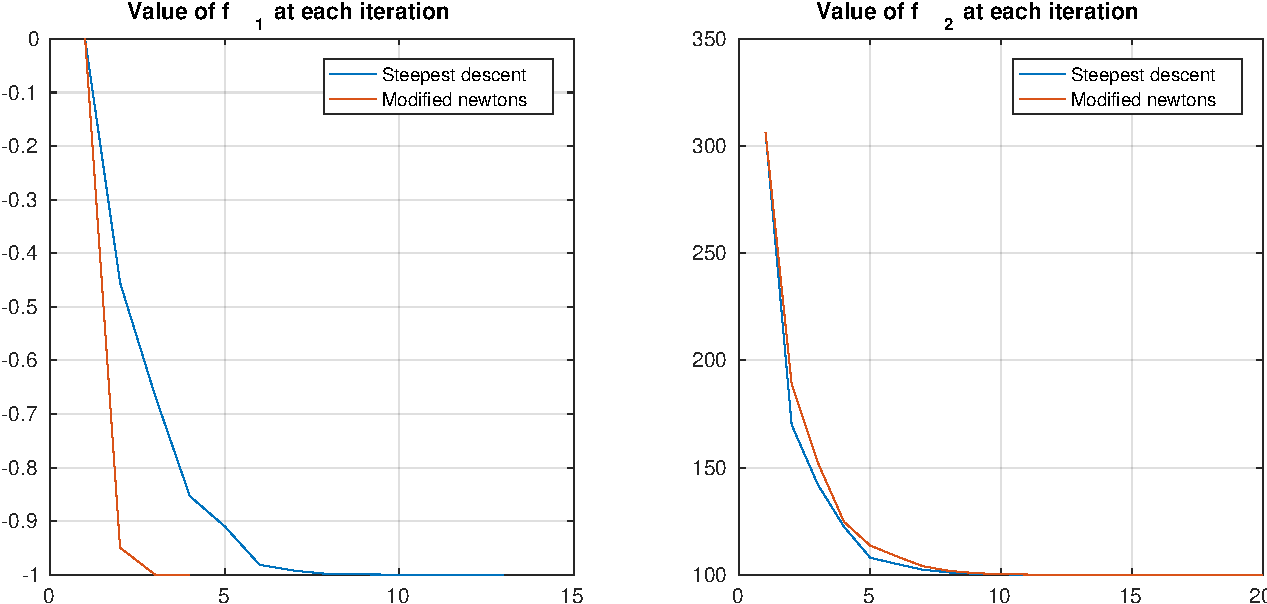
\includegraphics[width=\linewidth]{fig/unconstrained_exercices/pb7_1-crop}


\textbf{g)}

\answer

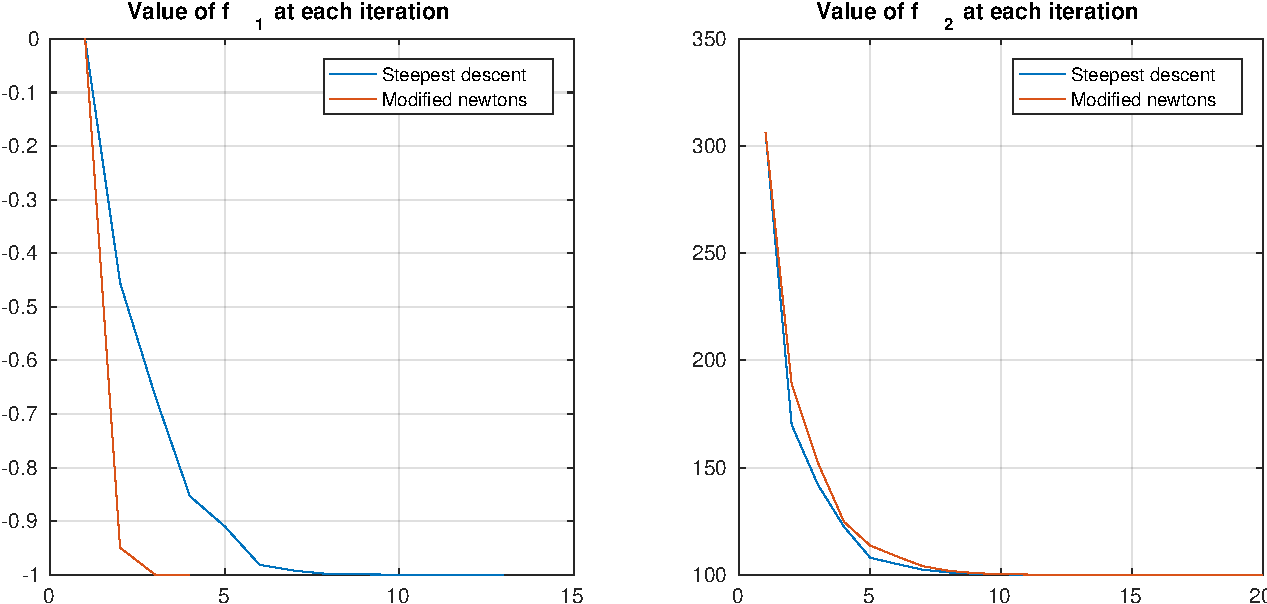
\includegraphics[width=\linewidth]{fig/unconstrained_exercices/pb7_1-crop}


\subsection{Problem 8}

\textbf{a)} 

\answer \footnote{\url{https://en.wikipedia.org/wiki/Broyden's_method}}


\[
	a = \frac{\Delta f_n - B_{k-1}s_k}{\| s_k\|^2}
\]

\textbf{b)}

\answer 

Chapter 6 p.144

We again want $B_{k+1}$ to satisfy the secant equation so 

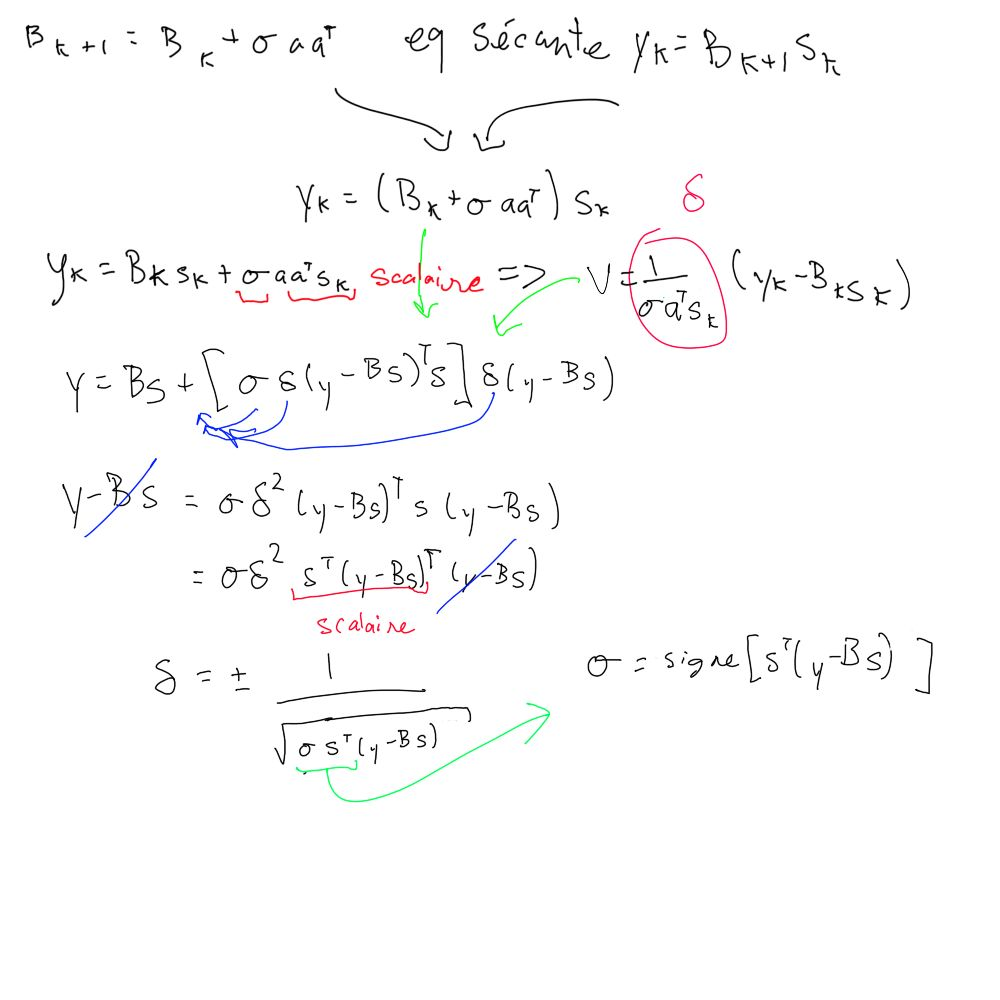
\includegraphics[scale=0.5]{fig/unconstrained_exercices/pb8_b}

\textbf{c)}

For some reason I just couldn't get the algebra to work out to $B_k$ :( ...

\subsection{Problem 9}

\textbf{a)}

\answer \footnote{\url{https://stanford.edu/class/ee364b/lectures/conj_grad_slides.pdf}}

Shifting? Solve $Ax = b - A\bar{x}$ using CG starting at $x_0 = 0$ and then from that solution solving the original $Ax = b$

\textbf{b)}

\answer

Je n'ai pas fait le cours de calcul scientifique...

\textbf{c)}

\incomplete

\textbf{d)}

\incomplete

\subsection{Problem 10}

\incomplete

\subsection{Problem 11}

\textbf{a)}

\answer

\[
	\nabla f(x) = A^T(Ax-b) = 0
\]

\textbf{b)}

$f(x)$ est convexe?

\answer

We know that $g(x) = x^2$ is convex and we know that $h(x) = \| x \|$ is convex and a composition of two convex functions $g(h(x))$ is also convex. Therefore $f(x)$ is convex. All that is left is to show that $Ax+b$ is convex.

\begin{align*}
	A(\lambda x + (1-\lambda )y) + b & \leq \lambda (Ax+b) + (1-\lambda ) (Ay+b) \\
	\lambda Ax + (1-\lambda) A y + b & \leq \lambda Ax + \lambda b + (1-\lambda)Ay + (1-\lambda)b \\
	\lambda Ax + Ay - \lambda A y + b &\leq \lambda Ax + \lambda b + Ay - \lambda A y + b - \lambda b \\
	\lambda Ax + Ay - \lambda A y + b &\leq \lambda Ax + Ay - \lambda A y + b \\
\end{align*}

CQFD

\textbf{c)}

\answer

Not necessarily. Depends on the shape of A.

\textbf{d)}

\answer

Conjugate gradient, modified newton's , quasi-newton

\textbf{e)}

\answer

\begin{align*}
	I_m r + Ax &= b \\
	A^T r &= 0
\end{align*}

$r$ is the "error" or the "residual" $r = Ax - b$, substitude that in and we get

\begin{align*}
	Ax -b + ax = b &\rightarrow Ax = b \\
	A^TAx - A^T b = 0 &\rightarrow A^T(Ax-b) = 0
\end{align*}

First eq is the system itself. Second eq is the first order optimality condition.

\textbf{f)}

\incomplete

\subsection{Problem 12}

\textbf{a)} Write first order optimality conditions

\answer

\[
	\nabla f(x) = A^T(Ax-b) + \lambda^2 x = 0
\]

\textbf{b)}

\answer

The sum of two convex functions is convex. We know the first part is convext now we need to show that the second part is. Through the same reasoning as in problem 11 we see that $\frac{1}{2} \lambda^2 \| x \| ^2$ is also convex. Therefore $f(x)$ is convex.

\textbf{c)}

\answer

If the rank of $A$ is less than $n$ then no.

\textbf{d)}

\answer

\[
	f(x) := \frac{1}{2} \| Ax - b + \lambda^2 x\|^2 - \langle\, Ax-b,x\rangle
\]


\textbf{e)}

\answer

Knowing that $r = Ax - b$
\begin{align*}
	I_m r + Ax = b &\rightarrow Ax = b \\
	A^T Ax - A^T b - \lambda^2 I x = 0 &\rightarrow A^T(Ax-b) - \lambda^2I_nx = 0
\end{align*}

First line is the system, second line is the first order optimality conditions.

\textbf{f)}

\answer

Proof using principal minors. All minors of $I_m$ are positive. Since $-\lambda^2 I_n$ is all negative. At some point when taking the principal minors we will get negative values. Since some minors are positive and some are negative, the matrix is indefinite.

\subsection{Problem 13}

\textbf{a)}

\answer

\[
J(x) = \begin{bmatrix}
	\frac{\partial f_1}{x_1} & \ldots & \frac{\partial f_m}{x_1} \\
	\vdots & \ddots & \vdots \\
	\frac{\partial f_1}{x_n} & \ldots & \frac{\partial f_m}{x_n} \\
\end{bmatrix}
\]

\textbf{b)}

\answer

Reuse answer from problem 4
\begin{align*}
	\nabla f(x) &= \nabla F(x)F(x)
\end{align*}

\color{red}
Answer from book

\[
	\nabla f(x) = J^T(x) F(x)
\]

\color{black}

\textbf{c)}

\answer

\[
	\nabla^2 f(x) = \nabla F(x) \nabla F(x) + F(x) \nabla^2F(x)
\]

\color{red}
Answer from book

\[
	\nabla^2 f(x) = J^T(x) J(x) + \sum_{j=1}^m F(_j(x) \nabla^2 F_j(x)
\]

\color{black}

\textbf{d)}

\answer

\begin{align*}
	d = - J^T(x) F(x) \Big( J^T(x) J(x) + \sum_{j=1}^m F(_j(x) \nabla^2 F_j(x)\Big)^{-1}
\end{align*}

\textbf{e)}

\answer

Maybe
\[
	d = - J^T(x) F(x) \Big( J^T(x) J(x))^{-1}
\]

\incomplete

\textbf{f)}

\incomplete

\subsection{Problem 14}

\textbf{a)}

\answer

Proof by contradiction

If the directions $p_j$ are not linearly independent then we can write $p_i$ as a linear combination of $p_j$
\[
	p_i = c_1 p_1 + \ldots + c_jp_j + \ldots + c_np_n
\]
Where $c_j \in \mathbb{R}$ and $j = {1, 2, \ldots, n}$ and $j \neq i$. We can then rewrite the equation
\begin{align*}
	p_i^T A p_j = 0 \\
	c_1p_1^TAp_j + \ldots + c_jp_j^TAp_j + \ldots + c_np_n^TAp_n = 0
\end{align*}

Since we know all the directions $p_j \neq 0$ then all the scalars $c_j$ must be 0. But this implies that the vectors are in fact not linearly dependent, which is a contradiction to our hypothesis. Therefore all directions are linearly independnt.

\textbf{b)}

\answer

Same as exercise in the unconstrained slides (48/71)

By definition $A \prec 0$ if all eigen values $\lambda$ are positive. Also by definition, $A$ is a linear transformation matrix on a vector $v$ such that $Av = \lambda v$. So we can rewrite the equation as
\begin{align*}
	p_i^TAp_i = p_i^T \lambda p_i &> 0 \\
	\lambda p_i^T p_i &> 0 \\
	\lambda \| p_i \|^2 &> 0
\end{align*}
Which can only be true if $\lambda > 0$. If all $\lambda$ have to be positive then $A \prec 0$.

\subsection{Problem 15}

\textbf{a)}

\answer

If $Q$ is orthogonal then $Q^TQ = I = QQ^T$ and $Q$ does not affect the euclidiean norm $\|x\| = \|Qx\|$ we can then substitute
\begin{align*}
	\| Ax - b \| &= \| Q\bar{R} -b \| \\
\intertext{Multiply the inside of the norm by $Q^T$}
	&= \|Q^TQ\bar{R} - Q^Tb\| \\
	&= \|\bar{R} - Q^Tb\|
\end{align*}

It's equivalent because the norm of an orthogonal matrix is $1$. So the two problems are equivalent/have the same solution.

\textbf{b)}

\textbf{b) i)}

\answer

$\text{rank}(R) = 3$ but $Q^Tb$ has $5$ rows. Also if you do the long multiplication you have
\begin{align*}
\frac{1}{2} \| \bar{R}x - Q^Tb\|^2 &=  \frac{1}{2}\|
\begin{bmatrix}
	x_1 + 2x_2 + 3x_3\\
	4x_2 + 5x_3\\
	6x_3 \\
	0 \\
	0 \\
\end{bmatrix}
-
\begin{bmatrix}
12 \\ 10 \\ 6 \\ \beta_4 \\ \beta_5
\end{bmatrix} \|\\
&= \frac{1}{2} \Bigg( (x_1 + 2x_2 + 3x_3 - 12)^2 + (4x_2 + 5x_3 -10)^2 + (6x_3 - 6)^2 + \beta_4^2 + \beta_5^2  \Bigg) \\
&=\frac{1}{2} \Bigg( (x_1 + 2x_2 + 3x_3 - 12)^2 + (4x_2 + 5x_3 -10)^2 + (6x_3 - 6)^2  \Bigg) + \frac{1}{2}( \beta_4^2 + \beta_5^2)
\end{align*}

From the last line we can see that whatever the answer for the values of $x$ turn out to be, the objective function will always have a positive number summed with the constant $\frac{1}{2}( \beta_4^2 + \beta_5^2)$.

We can generalize this result using formula 10.18 page 252 of the book

\begin{align*}
	\|Ax -b\|^2 &= \|\begin{bmatrix}
		Q_1^T \\ Q_2^T
	\end{bmatrix} A \Pi \Pi^Tx-b \|^2 \\
	&= \|\begin{bmatrix}
		R \\ 0
	\end{bmatrix} \Pi^Tx-\begin{bmatrix}
		Q_1^Tb \\ Q_2^Tb
	\end{bmatrix} \|^2 \\
	&= \| R\Pi^Tx-Q_1^Tb\|^2 + \|Q_2^Tb\|^2
\end{align*}

Where apparently 
\begin{enumerate}
\item $\Pi$ is an othogonal permutation matrix.
\item $Q_1$ is the first $n$ columns of Q
\item $Q_2$ is the rest of the columns of Q
\end{enumerate}

\textbf{b) i)}

\answer

If $\frac{1}{2} \Bigg( (x_1 + 2x_2 + 3x_3 - 12)^2 + (4x_2 + 5x_3 -10)^2 + (6x_3 - 6)^2  \Bigg) = 0$ then we can solve for $x$

\[
\begin{bmatrix}
	1 & 2 & 3 & -12 \\
	  & 4 & 5 & -10 \\
	  &   & 6 & -6
\end{bmatrix} =
\begin{bmatrix}
	1 & 2 & 3 & -12 \\
	  & 4 & 5 & -10 \\
	  &   & 1 & -1
\end{bmatrix} =
\begin{bmatrix}
	1 & 2 & 0 & -9 \\
	  & 4 & 0 & -5 \\
	  &   & 1 & -1
\end{bmatrix} =
\begin{bmatrix}
	1 & 0 & 0 & -\frac{13}{2} \\
	  & 4 & 0 & -5            \\
	  &   & 1 & -1
\end{bmatrix} =
\begin{bmatrix}
	1 & 0 & 0 & -\frac{13}{2} \\
	  & 0 & 1 & -\frac{5}{4}  \\
	  &   & 1 & -1
\end{bmatrix}
\]

$x_1 = -\frac{13}{2}$, $x_2 = -\frac{5}{4}$ and $x_3 = -1$

\textbf{c)}

\answer

(See page 252). We want to solve 
\begin{align*}
	\| R \Pi^T x^* - Q_1^Tb\|^2 &= 0 \\
	R \Pi^T x^* - Q_1^Tb &= 0 \\
	R \Pi^T x^* &= Q_1^Tb \\
\intertext{Since R is reversible}
	\Pi^T x^*  &= R^{-1}Q_1^Tb \\
\intertext{Since $\Pi$ is orthogonal}
	x^* &= \Pi R^{-1}Q_1^Tb
\end{align*}
	
\textbf{d)}

\answer

Knowing
\begin{align*}
	A = Q\bar{R} = \begin{bmatrix}
		Q1 & Q2
	\end{bmatrix} \begin{bmatrix}
		R \\ 0
	\end{bmatrix}\\
	A^T = \bar{R}^T Q^T = \begin{bmatrix}
		R^T & 0
	\end{bmatrix}\begin{bmatrix}
		Q1\\ Q2
	\end{bmatrix}
\end{align*}
We write
\begin{align*}
	A^T A z &= c \\
	\bar{R}^T Q^T Q\bar{R}z &= c \\
	\begin{bmatrix}
		R^T & 0
	\end{bmatrix}\begin{bmatrix}
		Q1\\ Q2
	\end{bmatrix} \begin{bmatrix}
		Q1 & Q2
	\end{bmatrix} \begin{bmatrix}
		R \\ 0
	\end{bmatrix} z &= c\\
	Q\begin{bmatrix}
		R \\ 0
	\end{bmatrix} z &= Q_1^{-1}R^{T^{-1}}c \\
	\begin{bmatrix}
		R \\ 0
	\end{bmatrix} z &= Q^TQ_1^{-1}R^{T^{-1}}c \\
\end{align*}

\subsection{Problem 16}

\answer

Say $ab^T = C$ some matrix $C$ then if we multiply both sides by a vector $d$

\begin{align*}
	a\textcolor{blue}{b^Td} = Cd	\\
\intertext{But the terms in blue result in a scalar so we can write}
	\left\langle b, d \right\rangle a = Cd
\end{align*}

If $C$ multiplied by $d$ is like multiplying a vector $a$ by a scalar then the rank of $C$ must be 1. 

\subsection{Problem 17}

\textbf{a)}

\answer

It's as if we had a series of points generated by $g(x)$ and we map each one of them by drawing segments to corresponding points on $p_n$ then we are trying to minimize the sum of these segments.

\textbf{b)}

\answer

First we can rewrite
\[
    p_n(x) = \sum_{i = 0}^{n}   a_i x^i
\]

Looks like the decision variables are the $a_i$ so the derivative is taken w.r.t. those coefficients.
\begin{align*}
    \frac{\partial f(x)}{\partial a_j} f(x) &= 2 \Bigg( \int_{0}^{1} g(x) - \sum_{i = 0}^{n}   a_i x^i dx \Bigg) \Bigg( \int_{0}^{1} g(x) - \sum_{i = 0}^{n}   a_i x^i dx \Bigg)'
\end{align*}

Tricky part, if you differentiate the polynomial $p_n$ by a certain $a_j$ then you're left with the corresponding $x^j$. So we can write
\[
    \frac{\partial}{\partial a_j} \sum_{i = 0}^{n}   a_i x^i = x^j \ \ \ \text{     where}\ \ \ \  j = \{0,1,\ldots,n\} 
\]
So now we can finish the differentiation
\begin{align*}
\frac{\partial f(x)}{\partial a_j} &= 2 \Bigg( \int_{0}^{1} g(x) - \sum_{i = 0}^{n}   a_i x^i dx \Bigg) (-x^j) \\
    &= 2 \Bigg( \int_{0}^{1} \sum_{i = 0}^{n}   a_i x^jx^i dx + \int_{0}^{1} x^j g(x) -  dx \Bigg) \\
\intertext{And we can take the sum out of the integral since it's a constant.}
    &= 2 \Bigg(  \sum_{i = 0}^{n}   a_i\int_{0}^{1} x^jx^i dx + \int_{0}^{1} x^j g(x) -  dx \Bigg)
\end{align*}

\textbf{c)}

\answer

So we have $g(x) = e^x$ and $p(x) = a_0 + a_1 x$

\begin{align*}
    f(x) &= \int_{0}^{1} \Big( e^x - a_0 - a_1 x\Big)^2 dx \\
    &= \int_{0}^{1} \Big( 
        e^{2x} - a_0e^x - a_1 x e^x
        -a_0 e^x + a_0^2 + a_0 a_1 x
        -a_1xe^x + a_0 a_1 x + a_1^2x^2    
    \Big) dx \\
    &= \int_{0}^{1} \Big( 
        e^{2x} - 2a_0e^x - 2a_1 x e^x
         + a_0^2 + 2a_0 a_1 x
          + a_1^2x^2    
    \Big) dx \\
    &= \frac{e^{x}}{2} - 2a_0e^x - 2a_1 e^x(x-1) + a_0^2 x + 2a_0 a_1 \frac{x^2}{2} + a_1^2 \frac{x^3}{3}\Bigg|_0^1 \\
    &= \frac{e^{1}}{2} - 2a_0e^1 - 2a_1 e^1(1-1) + a_0^2 + 2a_0 a_1 \frac{1^2}{2} + a_1^2 \frac{1^3}{3}\Bigg|_0^1 \\
    &= \frac{e^{1}}{2} - 2a_0e^1 + a_0^2 + a_0 a_1 + a_1^2 \frac{1}{3}
\end{align*}

First order necessary conditions

\[
    \nabla f(x) = 0\ \ \rightarrow\ \ \frac{\partial f(x)}{\partial a_0} = 0\ \ \text{and}\ \frac{\partial f(x)}{\partial a_1} = 0
\]
In other words

\begin{align*}
\begin{bmatrix}
    \frac{\partial f(x)}{\partial a_0} \\ 
    \frac{\partial f(x)}{\partial a_1}
\end{bmatrix} =
\begin{bmatrix}
    -2 \int_{0}^{1} \Big( e^x - a_0 - a_1 x\Big) dx \\
    -2 \int_{0}^{1} \Big( e^x - a_0 - a_1 x\Big)x dx
\end{bmatrix} &= 
\begin{bmatrix}
    0 \\ 0
\end{bmatrix} \\
\begin{bmatrix}
    -2 e^1 +2a_0 -a_1 \\
    -2 e^1(1-1) +a_0 + 2a_1 \frac{1^3}{3}
\end{bmatrix} &= 
\begin{bmatrix}
0 \\ 0
\end{bmatrix} \\
\begin{bmatrix}
-2 e^1 +2a_0  \\
a_0
\end{bmatrix} &= 
\begin{bmatrix}
a_1 \\ \frac{-2a_1}{3}
\end{bmatrix} \\
\begin{bmatrix}
-2 e^1 - \frac{4a_1}{3}  \\
a_0
\end{bmatrix} &= 
\begin{bmatrix}
a_1 \\ \frac{-2a_1}{3}
\end{bmatrix} \\
\begin{bmatrix}
-\frac{6 e^1}{7}  \\
a_0
\end{bmatrix} &= 
\begin{bmatrix}
a_1\\ \frac{-2a_1}{3}
\end{bmatrix} \\
\begin{bmatrix}
a_0 \\ a_1
\end{bmatrix} &= 
\begin{bmatrix}
 1.5533 \\ -2.3300
\end{bmatrix} 
\end{align*}

\textbf{d)}

\answer

We rewrite the objective as
\[
	f(x) = h \sum_{i=0}^n (g(x_i) - p(x_i))^2
\]

Our $g(x_i)$ is our constant $b$ and our $p(x_i)$ is what we want to optimize $Ax$ with decision variables $a_i$.

\begin{align*}
	h \|
	\begin{bmatrix}
		x^0 & x^1 & \ldots & x^n \\
		x^0 & x^1 & \ldots & x^n \\
		\vdots & \vdots & \vdots & \vdots\\
		x^0 & x^1 & \ldots & x^n \\
	\end{bmatrix}\begin{bmatrix}
		a_0 \\ a_1 \\ \vdots \\ a_n
	\end{bmatrix} - \begin{bmatrix}
		g(x_0) \\ g(x_1) \\ \vdots \\ g(x_N)
	\end{bmatrix}
	\|^2
\end{align*}

$A$ should have $N$ rows and $n$ columns








































\end{document}


